2016 was the hottest year on record since the beginning of weather recording in 1880~\cite{noaa}. Heat waves in summer and polar vortexes in winter are growing longer and pose increasing challenges to an already over-stressed electric grid. Furthermore, with the increasing penetration of renewable generation, the electricity grid is also experiencing a shift from predictable and dispatchable electricity generation to variable and non-dispatchable generation. This adds another level of uncertainty and volatility to the electricity grid. The volatility due to the mismatch between electricity generation and supply further leads to volatility in the wholesale price of electricity. For example, the polar vortex triggered extreme weather events in the U.S. in January 2014, which caused many electricity customers to experience increased costs. Parts of the U.S. north-eastern electricity grid experienced a 86-fold increase in the price of electricity from $\$31/\si{\mega\watt\hour}$ to $\$2,680/\si{\mega\watt\hour}$ in a matter of a few minutes~\cite{volatility}.  Such events show how unforeseen and uncontrollable circumstances can greatly affect electricity prices that impact grid operator and customers. Electricity price volatility, is becoming the new norm rather than the exception.

Across the United States, utilities and grid operators are devoting increasing attention and resources to Demand Response (DR). It is considered as a reliable means of mitigating the uncertainty and volatility of renewable generation and extreme weather conditions and improving the grid's efficiency and reliability. The resource contribution from all U.S. DR programs is estimated to be nearly 72,000 MW, or about 9.2 percent of U.S. peak demand~\cite{federal2008assessment} making DR the largest virtual generator in the U.S. national grid. The annual revenue to end-users from DR markets with PJM ISO alone is more than \$700 million~\cite{pjm}. Global DR revenue is expected to reach nearly \$40 billion from 2014 through 2023~\cite{navigant}.

The volatility in real-time electricity prices poses the biggest operational and financial risk for large scale end-users of electricity such as large commercial buildings, industrial and institutional customers (often referred to as \textit{C/I/I} consumers). In order to shield themselves from the volatility and risk of high prices, such consumers must be more flexible in their electricity demand. Consequently, large \textit{C/I/I} customers are increasingly looking to demand response programs to help manage their electricity costs. DR programs involve a voluntary response of a building to a price signal or a load curtailment request from the utility or the Curtailment Service Provider (CSP). Upon successfully meeting the required curtailment level the end-users are financially rewarded, but may also incur penalties for under-performing and not meeting a required level of load curtailment. In practice, one of the biggest challenges with end-user demand response is the following: \emph{Upon receiving the notification for a DR event, what actions must the end-user take in order to achieve an adequate and a sustained DR curtailment?} 

Unfortunately, most of the Demand Response today is done in an ad-hoc manner. 
The decisions are rule-based or they depend upon a building operator's experience, which has several disadvantages:

\begin{itemize}[leftmargin=0.5cm]
	\item \emph{Limitations of rule-based DR:} The building's operating conditions, internal thermal disturbances and environmental conditions must all be taken into account to make appropriate DR control decisions, which is not possible with using rule-based and pre-determined DR strategies since they do not account for the state of the building but are instead based on best practices and rules of thumb. 
	Rule based DR strategies have the advantage of being simple but they do not account for the state of the building and weather conditions during a DR event.
	\item \emph{Control complexity and scalability.} Upon receiving a notification for a DR event, the building's facilities manager must determine an appropriate DR strategy to achieve the required load curtailment. 
	These control strategies can include adjusting zone temperature set-points, supply air temperature and chilled water temperature set-point, dimming or turning off lights, decreasing duct static pressure set-points and restricting the supply fan operation \etc
	In a large building, it is difficult to assess the effect of one control action on other sub-systems and on the building's overall power consumption because the building sub-systems are tightly coupled.
\end{itemize}
These drawbacks are addressed by predictive control techniques such as Model Predictive Control (MPC). MPC allows to optimize desired performance while guaranteeing system's constraints. For example, it can be used to provide the optimal actions for an energy curtailment during a DR event while guaranteeing thermal comfort for occupants. So MPC-based solutions fit into the DR problem. However, the quality of the MPC solutions depends on the accuracy of the predictive models describing the system. This limits the widespread of MPC for complex systems such as buildings. Thus, in context of modeling of large buildings, applying MPC poses further challenges:

\begin{itemize}[leftmargin=0.5cm]
\item \emph{Modeling complexity and heterogeneity.} Unlike the automobile or the aircraft industry, each building is designed and used in a different way and therefore it must be uniquely modeled. Learning predictive models of building's dynamics using first principles based approaches (\eg with EnergyPlus~\cite{Crawley2001319}) is very cost and time prohibitive and requires retrofitting the building with several sensors~\cite{costmpc}. The user expertise, time and costs required to develop a model of a single building are very high.
%\item \emph{Interpretability of modeling and control.} Predictive models for buildings, regardless how sophisticated, lose their effectiveness unless they can be interpreted by human experts and facilities managers in the field. Therefore, the required solution must be transparent, human centric and highly interpretable.
\end{itemize}

\subsection{Main contribution}

In order to address the aforementioned challenges, we use machine learning algorithms to generate data-driven models for cyber-physical systems where we preserve predictive capability of model-based control but without the expense of first principle or grey-box model development.
Although machine learning algorithms are a popular choice for predicting systems' behavior, they do not provide models that are suitable for control.
In our previous work \cite{BehlJainMangharam2016,Behl201630}, we overcome this issue by using regression tree-based algorithms to provide models of system dynamics to be used in an optimal control problem setup.
%We  discussed the use of regression trees-based approaches to estimate the DR baseline power consumption and to build auto-regressive trees for DR control strategies evaluation.
%We further showed the procedure to design such a controller for energy management during Demand Response.
We proposed an algorithm for model-based control using regression trees (mbCRT), and apply it to synthesize real-time DR strategy.
The mbCRT algorithm can be used to setup optimal control problems with one-step lookahead prediction, for example to trade off thermal comfort inside a building against the amount of load curtailment.
However, mbCRT cannot be used to setup a receding horizon control problem with an arbitrarily length of the horizon as in MPC. 
This drawback limits the closed-loop control performance since it does not take into account the very accurate long term state prediction that regression trees can provide. 
In this paper, we overcome this issue providing the following contributions:

\begin{itemize}[leftmargin=0.5cm]
	\item \emph{Multi-variate regression trees:} We introduce a methodology to construct a multi-variate or multi-output predictive model using regression trees, where each output corresponds to the prediction on a future step of the horizon. More precisely, we setup a least square problem that minimize the prediction error over the control horizon. This is done by modifying the variable selection and splitting criteria at the nodes of the standard regression tree algorithm CART \cite{BreimanFriedmanStoneEtAl1984}.
	\item \emph{Predictive control:} We extend the mbCRT algorithm proposing a Data-driven Predictive Control strategy using Regression Trees (DPCRT), that implements receding horizon control using data-based models learned from the available historical data.
	\item \emph{Application:} We apply this control strategy to peak power curtailment on a large office building and compare with the previous mbCRT algorithm. Our results show an improvement of $8.6\%$ in terms of peak curtailment is obtained using DPCRT with respect to mbCRT.
\end{itemize}
In summary, the methodology proposed in this paper bypasses the cost and time prohibitive process of building high fidelity models (using grey and white box approaches) while still being suitable for receding horizon control. 
%These are the first algorithms of its kind that enable closed-loop control synthesis and finite receding horizon control with regression trees. 
The contributions of the paper are graphically shown in Fig. \ref{F:scheme}.

\subsection{Related work}
\label{sec:related}
In recent years, data-driven optimal control has drawn a huge interest in the research community.
Several different approaches have been considered. 
For example, in one approach, models are trained on optimal solutions obtained from MPC. 
The resulting models can then be used for explicit MPC, as in~\cite{BemporadMorariDuaEtAl2002}. This approach has been applied to problems of stabilization \cite{CavagnariMagniScattolini1999} and freeway traffic systems using regression trees \cite{OleariFrejoCamachoEtAl2015}. 
In applications like buildings, where obtaining a model for MPC is hard, such techniques cannot be used.
Another class of methods solve the optimization directly on the trained models to do predictive control \cite{Hou2013,Costanzo2016,FerreiraRuanoSilvaEtAl2012}. 
However, none of them addresses the problem of including data-driven state models into the optimal predictive control loop. Hence, we cannot solve an MPC-like optimal control problem. 
In \cite{Behl201630}, we proposed MPC-like control problem considering regression tree-based algorithms for the DR problem. In \cite{KusiakSongZheng2009}, neural networks are used instead to setup an MPC-like control for the wind turbine problem using evolutionary algorithms. Nevertheless, their approaches considered only one-step lookahead predictive model, and hence does not allow predictive control over an arbitrary horizon.

There is a vast literature more specific to the Demand Response which look at the problem of determining DR strategies \cite{oldewurtel2013towards,xu2004peak}. 
The majority of the approaches are either rule-based techniques for curtailment or white/grey box model-based control. 
These usually assume that the model of the system is well known whereas the task is much more complicated and time consuming in the case of a real building and sometimes, it can be even more complex and involved than the design of the controller itself. 
After several years of work on using first principles based models for demand response, multiple authors~\cite{costmpc,reallife} have concluded that the biggest hurdle to mass adoption of intelligent building control is the cost and effort required to capture accurate dynamical models of the buildings. 
There are ongoing efforts to make tuning and identifying white box models of buildings more autonomous~\cite{new2012autotune}. 
OpenADR standard and protocol~\cite{openadr} describes the formats for information exchange to facilitate DR but modeling, prediction and control strategies are out of scope. 
Several machine learning approaches~\cite{edwards2012predicting,vaghefi2014modeling,yin2012scalable} have been utilized before for forecasting electricity load including some which use regression trees. 
However, there are two significant shortcomings of the work in this area: 
	\begin{inparaenum}[(a)]
		\item these approaches are coarse grained and  are not aimed at solving demand response problems but are restricted to long term load forecasting with applications in evaluating building retrofits savings and building energy ratings, and
		\item  there is no focus on control synthesis or addressing the suitability of the model to be used in control design. 
	\end{inparaenum}
	There exist several different approaches to balance the power consumption in buildings and avoid peaks, e.g. by load shifting and load shedding \cite{KiliccoteEtAl06aca,LeeEtAl08dom}. However, they operate on coarse grained time scales and do not guarantee any thermal comfort.

\begin{figure}[t!]
	\begin{center}
		\hspace{0.8cm}
		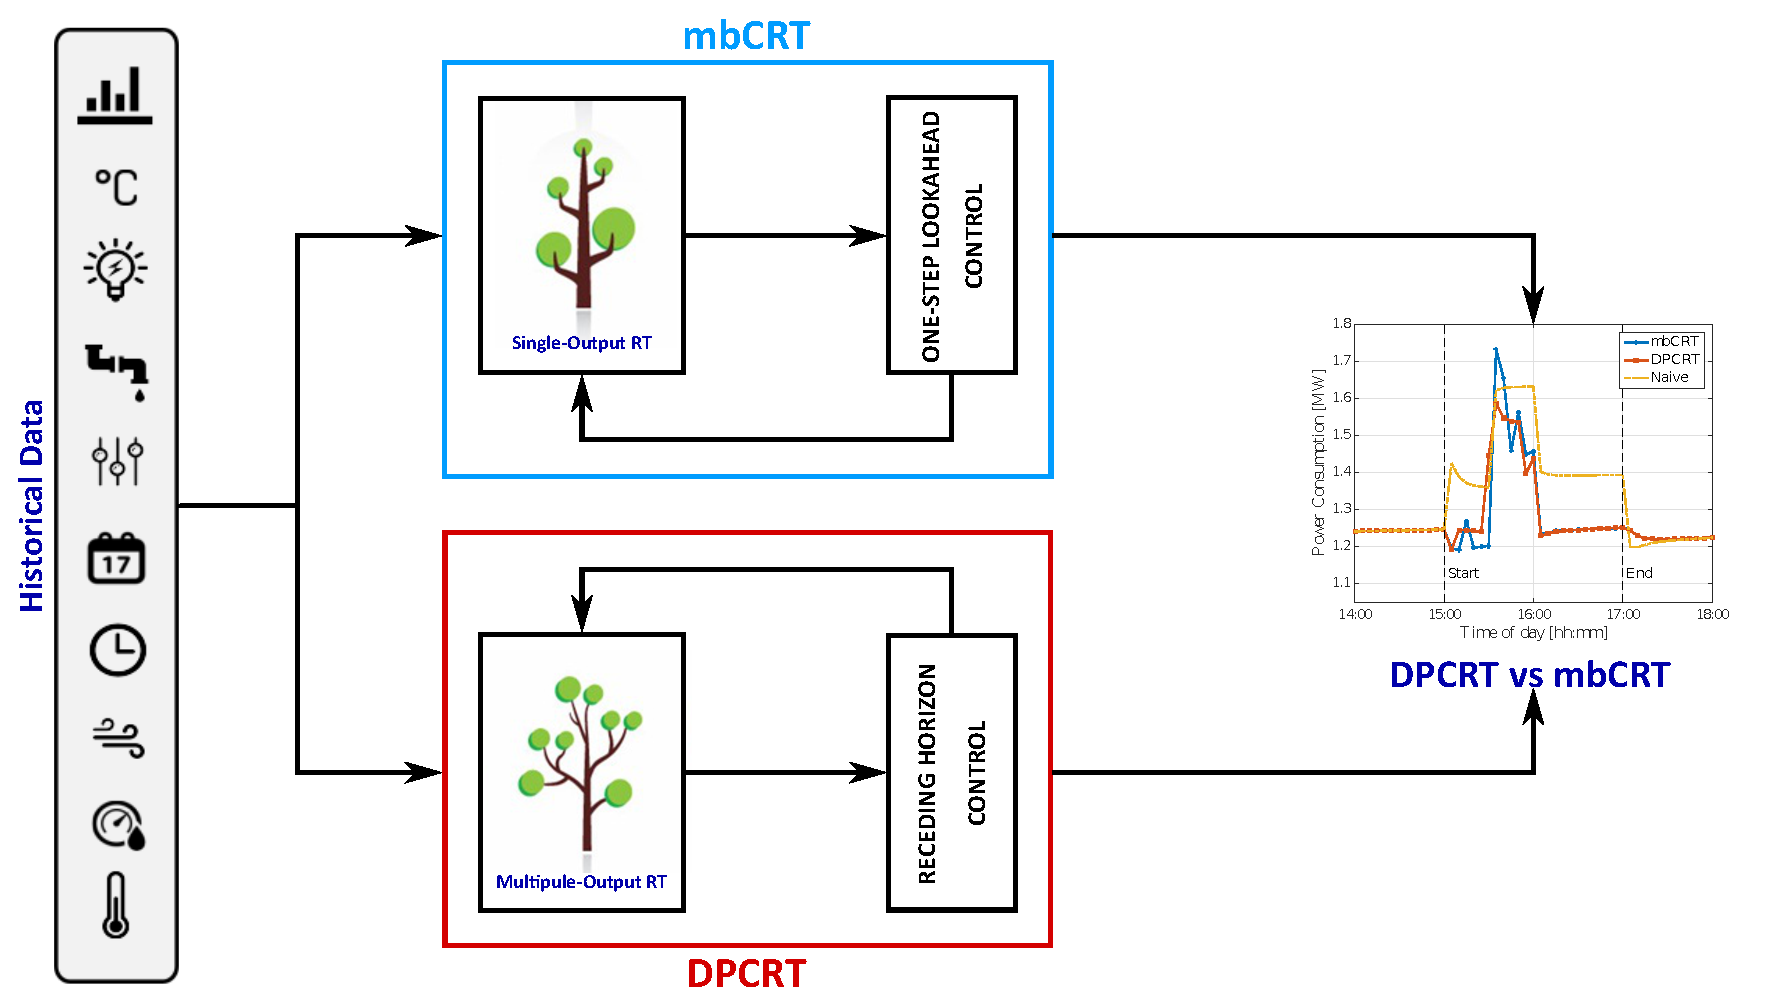
\includegraphics[width=0.8\textwidth]{Figures/scheme.eps}
		\centering
		\caption{Historical data are used to train models for mbCRT in Sec.~\ref{sec:drtree} and DPCRT in Sec.~\ref{sec:decision_tree}. These models are then used in the optimization in a closed-loop with the physical system. Finally, the two approaches are compared in Sec~\ref{sec:case}.}
		\label{F:scheme}
		\vspace{-10pt}
	\end{center}
\end{figure}

The DPCRT algorithm is first of its kind that does finite receding horizon control with regression trees. 
It is computationally efficient because the optimization problem is convex and the number of constraints scales linearly with the number of control variables. 
A preliminary version of this paper can be found in the conference paper \cite{JainBuildsys2016}.

\subsection{Paper organization}

This paper is organized as follows. We describe our problem formulation in Sec.~\ref{sec:problem}. 
Sec.~\ref{sec:drtree} provides an overview of the data-driven control strategy (mbCRT) proposed in \cite{Behl201630} that will be useful to introduce our new methodology. 
In Sec.~\ref{sec:decision_tree}, we present our main contribution -- predictive control using multi-variate regression trees. 
In particular, we extend the standard training algorithm for regression trees in Sec. \ref{SS:training_algo} so we can use it to build predictive models over a horizon of arbitrary length. 
In Sec. \ref{SS:control_tree}, we use the DPCRT algorithm to formally build system models and setup a receding horizon optimal control problem that can be used for the closed-loop control. 
Finally, in Sec. \ref{sec:case} we apply DPCRT to a peak power reduction problem and compare it with mbCRT.

